% !TeX spellcheck = ru_RU
% !TEX root = vkr.tex

\section{Демонстрационная база данных}

В данном разделе продемонстрированы:
\begin{itemize}
    \item шаги создания демонстрационной базы данных;
    \item информация о предварительной обработке текста и его загрузки в СУБД;
    \item реализация Docker-образа~\cite{DockerDocs}.
\end{itemize}

\subsection{Проектирование и создание таблицы}

Отношение между автором и текстом --- это связь \enquote{один-к-одному}, поэтому достаточно создать одну таблицу и заполнить ее необходимым данными.
Представление таблицы на физическом уровне представлено на рисунке~\ref{schema}.

\begin{figure}[H]
    \centering
    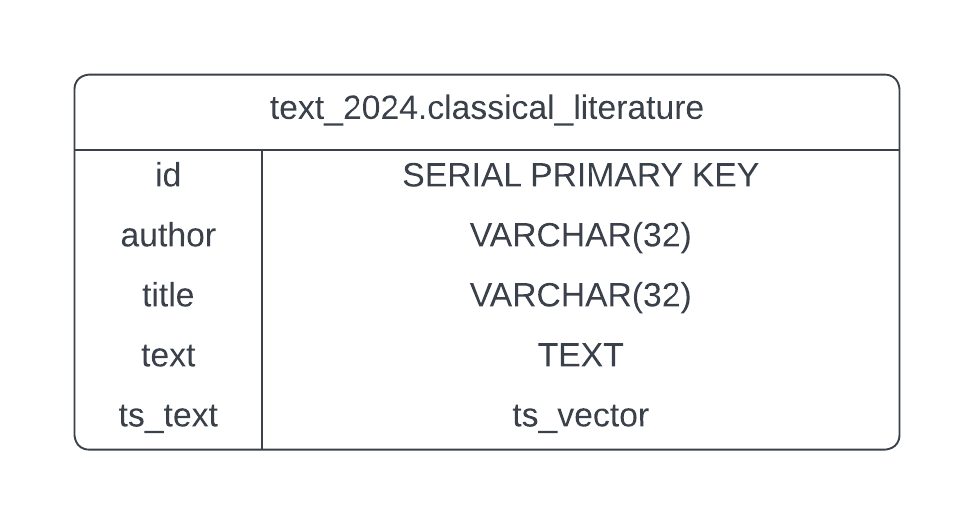
\includegraphics[width=\textwidth, scale=0.85]{figures/er-diagram}
    \caption{Схема базы данных}
    \label{schema}
\end{figure}

В листинге~\ref{init-db} продемонстрированы команды для создания таблицы.

\begin{algorithm}[H]
    \floatname{algorithm}{Листинг}
    \caption{Код SQL для создания таблицы}
    \label{init-db}
    \begin{lstlisting}[style=codelistingstyle]
      CREATE TABLE IF NOT EXISTS text_2024.classical_literature(
            id SERIAL,
            author character varying(32) NOT NULL,
            title character varying(32) NOT NULL,
            text TEXT NOT NULL
      );

      ALTER TABLE text_2024.classical_literature
            ADD CONSTRAINT pk_classical_literature PRIMARY KEY (id);

      ALTER TABLE text_2024.classical_literature ADD column ts_text tsvector;

      UPDATE text_2024.classical_literature
            SET ts_text = to_tsvector(
                  'russian',
                  text_2024.classical_literature.text
      );
      \end{lstlisting}
\end{algorithm}

\subsection{Подготовка текстовых данных}

Было отобрано 21 произведение классической литературы.
Тексты произведений взяты из открытого банка ФИПИ\footnote{\href{https://ege.fipi.ru/bank/index.php?proj=B9ACA5BBB2E19E434CD6BEC25284C67F}{Дата обращения \DTMdate{2024-09-15}: Открытый банк ФИПИ заданий ЕГЭ по информатике}} по информатике (фильтр по заданию с кодификатором $4.6$ \enquote{Текстовый процессор}).
Информация об отобранных текстах представлена в таблице~\ref{text-data}.
Подсчет слов был произведен утилитой \texttt{wc}.

\begin{longtable}{|c|l|l|l|}
    \hline
    \textbf{№} & \textbf{Автор} & \textbf{Название} & \textbf{\# слов}   \\ \hline
    1  & Булгаков М.А.    & Собачье сердце                      & 26033  \\ \hline
    2  & Лермонтов М.Ю.   & Герой нашего времен                 & 43200  \\ \hline
    3  & Некрасов Н.А.    & Кому на Руси жить хорошо            & 31893  \\ \hline
    4  & Чехов А.П.       & Человек в футляре                   & 4142   \\ \hline
    5  & Бах Р.Д.         & Чайка по имени Ливингстон           & 8426   \\ \hline
    6  & Стругацкие       & Понедельник начинается в субботу    & 60779  \\ \hline
    7  & Булгаков М.А.    & Мастер и Маргарита                  & 118013 \\ \hline
    8  & Гоголь Н.В.      & Вечера на хуторе близ Диканьки      & 63657  \\ \hline
    9  & Грин А.С.        & Алые Паруса                         & 20502  \\ \hline
    10 & Киплинг Д.Р.     & Маугли                              & 49554  \\ \hline
    11 & Куприн А.И.      & Поединок                            & 68311  \\ \hline
    12 & Лермонтов М.Ю.   & Мцыри                               & 3380   \\ \hline
    13 & Платонов А.П.    & Юшка                                & 2300   \\ \hline
    14 & Пушкин А.С.      & Дубровский                          & 21564  \\ \hline
    15 & Пушкин А.С.      & Евгений Онегин                      & 22649  \\ \hline
    16 & Пушкин А.С.      & Капитанская дочка                   & 30287  \\ \hline
    17 & Толстой Л.Н.     & Анна Каренина                       & 280023 \\ \hline
    18 & Толстой Л.Н.     & Севастопольские рассказы            & 36539  \\ \hline
    19 & Хемингуэй Э.М.   & Прощай оружие                       & 79316  \\ \hline
    20 & Чехов А.П.       & Воры                                & 4996   \\ \hline
    21 & Грин А.С.        & Бегущая по волнам                   & 57994  \\ \hline
    \caption{Список авторов и произведений}
    \label{text-data}
\end{longtable}

Для упрощения загрузки текстовых данных в СУБД была проведена предварительная очистка текста от несущественной информации (комментарии автора, оглавление, служебная информация редакции и т.п.).
Кроме того, из текста удалены символы переноса строки.
То есть весь текст представляет собой последовательность слов и символов, расположенных в одной строке.
Также ковычки заменены на двойной знак~\texttt{'}.
Это сделано для упрощения загрузки текстовых данных в Docker-контейнер при помощи \texttt{bash}-скрипта, срабатываемого автоматически при инициализации.

\subsection{Docker}

Контейнеризация реализована следующим образом.
В файле \texttt{compose.yaml} содержится рецепт запуска двух сервисов:
\begin{itemize}
    \item Docker-образ с PostgreSQL;
    \item Docker-образ с pgadmin4.
\end{itemize}

\noindent Оба сервиса связываются друг c другом через \texttt{docker network}.
После запуска контейнеров командой \texttt{docker compose up}~\cite{DockerComposeDocs} пользователь получает доступ к базе данных через локальный сервер по адресу \texttt{localhost:5050}.

\subsection{Загрузка текстовых данных в таблицу}

Для загрузки подготовленных произведений в СУБД на удаленном сервере использован \texttt{python}-скрипт.
Для создания таблицы и ее наполнения в Docker-контейнере написан \texttt{bash}-скрипт, который автоматически срабатывает во время развертывания контейнеров.
Все использованные скрипты доступны в репозитории\footnote{\href{https://github.com/artem-burashnikov/postgresql-fulltext-search}{Дата обращения \DTMdate{2024-09-15}: https://github.com/artem-burashnikov/postgresql-fulltext-search}}.

% \subsection{Некоторые типичные ошибки}
% Здесь мы будем собирать основные ошибки, которые случаются при написании текстов.
% В интернетах тоже можно найти коллекции типич\-ных косяков%
% \footnote{\href{https://www.read.seas.harvard.edu/~kohler/latex.html}{https://www.read.seas.harvard.edu/\textasciitilde kohler/latex.html} (дата обращения: \DTMdate{2022-12-16}).}.

% Рекомендуется по-умол\-ча\-нию использовать красивые греческие бук\-вы $\sigma$  и $\phi$, а именно $\phi$ вместо $\varphi$.
% В данном шаблоне команды для этих букв переставлены местами по сравнению с ванильным \TeX'ом.

% Также, если работа пишется на русском языке, необходимо, чтобы работа была написана на \textit{грамотном} русском языке даже если автор из ближнего зарубежья%
% \footnote{Теоретически, возможен вариант написания текстов на английском языке, но это необходимо обсудить в первую очередь с научным руководителем.}.
% Это включает в себя:
% \begin{itemize}
%     \item разделы должны оформляться с помощью \verb=\section{...}=, а также \verb=\subsection= и т.~п.; не нужно пытаться нумеровать вручную;
%     \item точки после окончания предложений должны присутствовать;
%     \item пробелы после запятых и точек, в конце слова перед скобкой;
%     \item неразрывные пробелы там, где нужны пробелы, но переносить на другую строку нельзя, например \verb=т.~е.=, \verb=А.~Н.~Терехов=, \verb=что-то~\cite{?}=, \verb=что-то~\ref{?}=;
%     \item дефис там, где нужен дефис (обозначается с помощью одиночного \enquote{минуса} (англ. dash) на клавиатуре);
%     \item двойной дефис там, где он нужен; а именно  при указании проме\-жутка в цифрах: в 1900--1910 г.~г., стр. 150--154;
%     \item тире (т.~е. \verb=---=~--- тройной минус) на месте тире, а не что-то другое; в русском языке тире не может \enquote{съезжать} на новую строку, поэтому стоит использовать такой синтаксис: \verb=До~--- после=;
%     \item даты стоит писать везде одинаково; чтобы об этом не следить, можно пользоваться заклинанием \verb=\DTMdate{2022-12-16}=;
%     \item правильные кавычки должны набираться с помощью пакета \texttt{csquotes}: для основного языка в \texttt{polyglossia} стоит использовать команду \verb=\enquote{текст}=, для второго языка стоит использовать \verb=\foreignquote{язык}{текст}=; правильные кавычки в русской типографии~--- \verb=<<ёлочки>>=, ни в коем случае не \verb="скандинавские лапки"=;
%     \item все перечисления должны оформляться с помощью \verb=\enumerate= или \verb=\itemize=; пункты перечислений должны либо начинаться с заглавной буквы и заканчиваться точкой, либо начинаться со строчной и закачиваться точкой с запятой; последний пункт пере\-числений всегда заканчивается точкой.
%     \item Перед выкладыванием финальной версии необходимо просмотреть лог \LaTeX'a, и обратить внимание на сообщения вида \emph{Overfull \textbackslash hbox (1.29312pt too wide) in paragraph}. Обычно, это означает, что текст выползает за поля, и надо подсказать, как правильно разделять слова на слоги, чтобы перенос произошел автоматически.
%           Это делается, например, так: \verb=соломо\-волокуша=.
%     \item \emph{Обязательно используйте инструменты автоматической проверки правописания!}
%           Не посылайте текст даже научному руководителю на проверку, если не прогнали спеллчекер%
%           \footnote{Например, для браузера можно использовать плагин LanguageTool, для VS Code --- Code Spell Checker с расширением для русского (но он вроде не умеет пунктуацию, так что следите за запятыми).}%
%           , желательно, умеющий проверять пунктуацию~--- у научника куча времени уйдёт на комментарии вида \enquote{тут нужна запятая} и не останется сил посоветовать что-нибудь по делу.
%           А ещё научник будет шокирован уровнем грамотности современной молодёжи, впадёт в депрессию и не будет отвечать вам неделю.
% \end{itemize}

% \subsection{Листинги, картинка и прочий \enquote{не текст}}

% Различный \enquote{не текст} имеет свойство отображаться не там, где он написан в текстовом виде в \LaTeX{}, поэтому у него должна быть самодостаточ\-ная понятная подпись \verb=\caption{...}=, уникальная метка \verb=\label{...}=, чтобы на неё можно было бы ссылаться в тексте с помощью \verb=\ref{...}= (более того, ссылка из текста обязательна).
% Ниже Вы сможете увидеть таблицу \ref{time_cmp_obj_func}, на которую мы сослались буквально только что.

% \enquote{Не текста} может быть довольно много~--- чтобы не засорять корневую папку, хорошим решением будет складывать весь \enquote{не текст} в папку \texttt{figures}.
% Заклинание \verb=\includegraphics{}= уже знает этот путь и будет искать там файлы без указания папки.
% Команда \verb=\input{}= умеет ходит по путям, например \verb=\input{figures/my_awesome_table.tex}=.
% Кроме того, листинги кода можно подтягивать из файла с помощью команды \verb=\inputminted{file}=.

% %% Вставка кода с помощью listings
% % \begin{lstlisting}[caption={Название для листинга кода. Достаточно длинное, чтобы люди, которые смотрят картинку сразу после названия статьи (т.~е. все люди), смогли разобраться и понять к чему в статье листинги, картинки и прочий \enquote{не текст}.}, language=Caml, frame=single]
% %   let x = 5 in x + 1
% % \end{lstlisting}

% %% Вставка кода с помощью minted
% \begin{listing}
%     \caption{Название для листинга кода. Достаточно длинное, чтобы люди, которые смотрят картинку сразу после названия статьи (т.~е. все люди), смогли разобраться и понять к чему в статье листинги, картинки и прочий \enquote{не текст}.}
%     \begin{minted}[frame=single]{ocaml}
%     let x = 5 in x + 1
%   \end{minted}
% \end{listing}

% \subsubsection{Выделение куска листинга с помощью tikz}
% Это бывает полезно в текстах, а ещё чаще~--- в презентациях.
% Пример сделан на основе вопроса на \textsc{StackExchange}%
% \footnote{Вопрос про рамку вокруг листинга на StackExchange, \url{https://tex.stackexchange.com/questions/284311} (дата обращения: \DTMdate{2022-12-16}).}.
% Заодно тут показывается альтернативный minted пакет, lstlistings, если не хотите ставить Python и пакет pygments.
% В этом случае закомментируйте всё, что связано с minted, в matmex-diploma-custom.cls.
% И внимательно следите за тем, чтобы везде использовался либо только lstlistings, либо minted~--- смешивание их в одном документе приведёт к странным ошибкам.

% \begin{figure}
%     % TODO(Kakadu): Сделать \lstset глобально, чтобы не выписывать все опции листингов каждый раз
%     \begin{lstlisting}[ escapechar=!, keepspaces=true, extendedchars=\true, texcl=true
%                       , basicstyle=\ttfamily, commentstyle=\color{eclipseGreen}\ttfamily\itshape, language=c ]
% #include <stdio.h>
% #include <math.h>

% /** A comment in English */
% int main(void)
% {
%   double c = -1;
%   double z = 0;

%   // Это комментарий на русском языке
%   printf ("For c = %lf:\n", c);
%   for (int i = 0; i < 10; i++ ) {
%     printf( !\tikzmark{a}!"z %d = %lf\n"!\tikzmark{b}!, i, z);
%     z = pow(z, 2) + c;
%   }
% }
% \end{lstlisting}

%     \begin{tikzpicture}[use tikzmark]
%         \draw[fill=gray,opacity=0.1]
%         ([shift={(-3pt,2ex)}]pic cs:a)
%         rectangle
%         ([shift={(3pt,-0.65ex)}]pic cs:b);
%     \end{tikzpicture}
%     \caption{Пример листинга c помощью пакета \texttt{listings} и \textsc{TIKZ} декорации к нему, оформленные в окружении \texttt{figure}.
%         Обратите внимание, что рисунок отображается не там, где он в документе, а может \enquote{плавать}.}
% \end{figure}

% \subsection{Некоторые детали описания реализации}
% Описание реализации~--- очень важный раздел для будущих программных инженеров, т.е. почти для всех.
% Важно иметь всегда, даже если Вы написали прототип на коленке или немного скриптов.

% В процессе работы можно сделать огромное количество косяков, неполный список которых ниже.

% \begin{enumerate}
%     \item Реализация должна быть.
%           На публично доступную реализацию обязательна ссылка (в заключении, но можно продублировать тут).
%           Если код под \textsc{NDA}, то об этом, во-первых, должно быть сказано явно,
%           во-вторых, на защиту должны выно\-ситься другие результаты (например, архитектура), чтобы комис\-сия имела возможность оценить хоть что-то,
%           и, в третьих, должна быть справка от работодателя, что Вы правда что-то сделали.
%           \begin{itemize}
%               \item Рецензент обязан оценить код (о возможности должен побеспо\-коиться обучающийся).
%           \end{itemize}
%     \item Код реализации должен быть написан защищающимся целиком.
%           \begin{itemize}
%               \item Если проект групповой, то нужно явно выделить, какие части были модифицированы защищающимся.
%                     Например, в преды\-дущих разделах на картинке архитектуры нужно выделить цветом то, что Вы модифицировали.
%               \item Нельзя пускать в негрупповой проект коммиты от других людей, или людей не похожих на Вас.
%                     Например, в 2022 году защищающийся-парень делал коммиты от сценического псев\-донима, который намекает на женский \enquote{гендер}.
%                     (Нет, это не шутка.)
%                     На тот момент в российской культуре это выглядело странно.
%               \item Возможна ситуация, что вы используете конкретный ник в интернете уже лет пять, и желаете писать ВКР под этим ником на \GitHub{}.
%                     В принципе, это допустимо, но если Вы встретите преподавателя, который считает наоборот, то Вам придется грамотно отмазы\-ваться.
%                     В Вашу пользу могут сыграть те факты, что к нику на \GitHub{} у Вас приписаны настоящие имя и фамилия; что в репозитории у вас видна домашка за первый курс;
%                     и что Ваш преподаватель практики сможет подтвердить, что Вы уже несколько лет используете это ник; и т.п.
%           \end{itemize}
%     \item Если Вы получаете диплом о присвоении квалификации программиста, код должен соответствовать.
%           \begin{enumerate}
%               \item Не стоит выкладывать код одним коммитом.
%               \item Не стоит выкладывать код аккурат перед защитой.
%               \item Лучше хоть какие-то тесты, чем совсем без них.
%                     В идеале нужно предъявлять процент покрытия кода тестами.
%               \item Лучше сделать \textsc{CI}, а также \textsc{CD}, если оно уместно в Вашем проекте.
%               \item Не стоит демонстрировать на защите, что Вам даже не пришло в голову напустить на код линтеры и т.п.
%           \end{enumerate}
%     \item Если ваша реализация по сути является прохождением стандартного туториала,
%           например, по отделению картинок кружек от котиков с помощью машинного обучения, то необходимо срочно сообщить об этом руководителю практики/ВКР,
%           иначе Государственная Экзаменацион\-ная Комиссия \enquote{порвёт Вас как Тузик грелку}, поставит \enquote{единицу},
%           а все остальные Ваши сокурсники получат оценку выше.
%           (Это не шутка, а реальная история 2020 года.)
% \end{enumerate}

% \noindent Если Вам предстоит защищать учебную практику, а эти рекомендации видятся как более подходящие для защиты ВКР, то ... отмаза не засчиты\-вается, сразу учитесь делать нормально.
